\bexo
Soit

\begin{equation}
	f(x) = 2x+1
	~~,~~
	g(x) = sin(x-\frac{\pi}{2})
\end{equation}

Tracer $h_1(x) = (f\circ g)(x)$ et $h_2(x) = (g \circ f)(x)$.

\begin{center}
	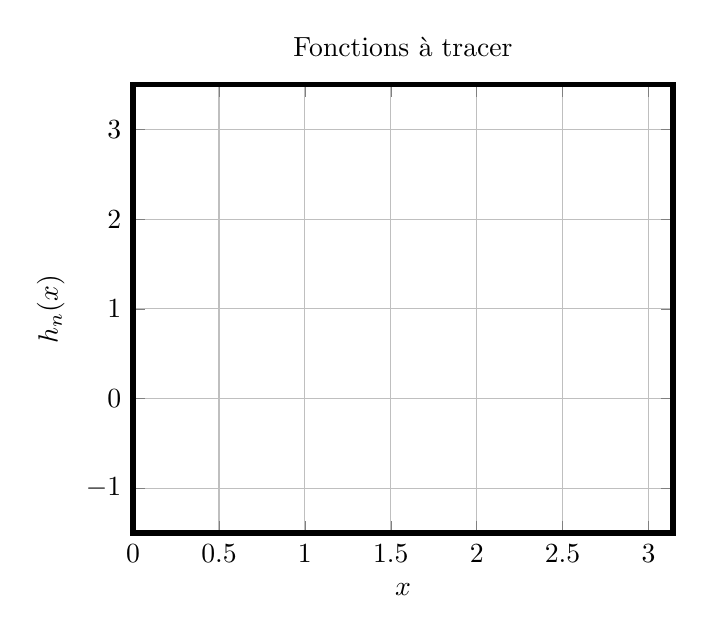
\begin{tikzpicture}
		\begin{axis}[
			line width=2pt,
			legend columns=-1,
			title=Fonctions à tracer,
			xlabel={$x$},
			ylabel={$h_n(x)$},
			xmin=0,
			xmax=pi,
			ymin=-1.5,
			ymax=3.5,
			legend to name=named,
			grid=major]
		\end{axis}
	\end{tikzpicture}
\end{center}
\eexo

\solution{\hfill\\
	Les graphes des fonctions sont:
	\begin{center}
		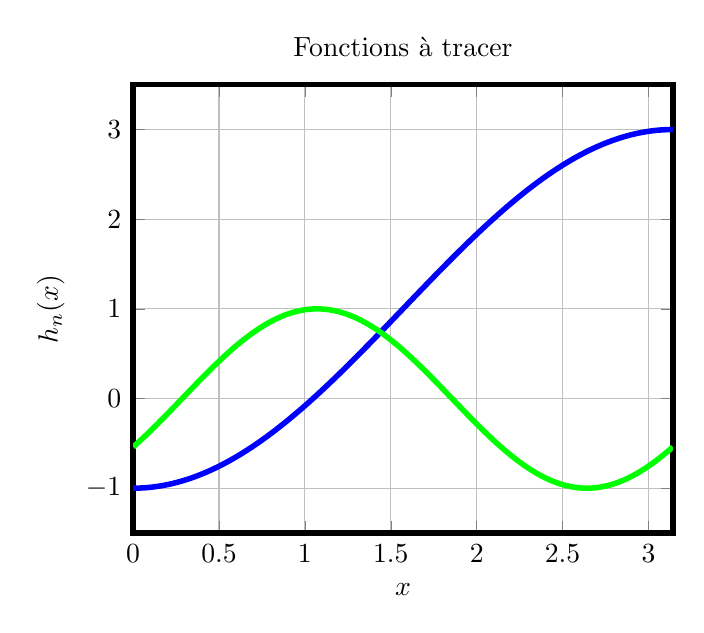
\begin{tikzpicture}
			\begin{axis}[
				line width=2pt,
				legend columns=-1,
				title=Fonctions à tracer,
				xlabel={$x$},
				ylabel={$h_n(x)$},
				xmin=0,
				xmax=pi,
				ymin=-1.5,
				ymax=3.5,
				legend entries={$h_1(x)$, $h_2(x)$},
				legend to name=named,
				grid=major]
			\addplot[blue,samples=500] expression[domain=0:pi]{2*sin(180*x/pi-90)+1};
				\addplot[green,samples=500] expression[domain=0:pi]{sin(180*(2*x+1)/pi-90)};
			\end{axis}
		\end{tikzpicture}
		\ref{named}
	\end{center}
}
